\documentclass{article}
\usepackage{graphicx}
\usepackage{hyperref}
\usepackage{amsmath, amssymb}
\usepackage{listings}
\usepackage{xcolor}
\usepackage{tikz}
\usetikzlibrary{positioning}

\title{OmniMCP: A Framework for Self-Generating UI Understanding Through Spatial-Temporal Synthesis}
\author{Richard Abrich \\ OpenAdapt.AI}
\date{March 2025}

\begin{document}

\maketitle

\begin{abstract}
We present OmniMCP, a novel framework that enables large language models to develop comprehensive UI understanding through the synthesis of spatial and temporal features. The framework combines fine-grained UI segmentation with process graphs derived from human demonstrations to construct rich contextual representations of interface states and interaction patterns. Our approach introduces a self-generating comprehension engine that bridges the gap between raw UI elements and task-specific interaction strategies. Through advanced prompt templates and synthetic validation techniques, we demonstrate robust understanding across diverse interface patterns.

% Our experimental results show [X]\% improvement in task completion rates across [Y] different UI patterns compared to baseline approaches. The framework demonstrates particular effectiveness in [specific use case], achieving [metric] performance. Key technical innovations include [innovation 1] and [innovation 2].

\end{abstract}

\section{Introduction}
User interface automation remains a significant challenge in artificial intelligence, particularly in developing systems that can generalize across diverse interfaces and adapt to varying contexts. While recent advances in computer vision and natural language processing have improved UI element detection, existing approaches often lack the ability to synthesize spatial understanding with temporal interaction patterns.

This paper introduces OmniMCP, a framework that addresses these limitations through two key mechanisms:
\begin{itemize}
    \item Real-time UI structure analysis via OmniParser
    \item Temporal pattern learning through process graph representations
\end{itemize}

\section{Related Work}
The challenge of automating interactions with user interfaces has been addressed through multiple paradigms over the past four decades, evolving from rudimentary screen parsing to sophisticated AI-driven approaches. We review key developments that form the foundation for our work on spatial-temporal synthesis for UI understanding.

\subsection{Conventional UI Automation Techniques}
Early UI automation relied primarily on brittle pixel-based matching and fixed coordinate systems \cite{chen2018}. These methods proved highly sensitive to visual variations, with even minor UI adjustments breaking automation scripts. The evolution continued with record-and-playback tools in the 1980s-1990s that captured user actions for later replay \cite{memon2003}. While accessible to non-programmers, these tools lacked the flexibility to handle dynamic interfaces.

Script-based tools emerged in the late 1990s, introducing programmatic control through specialized languages and APIs. This period saw the development of framework-based approaches that offered reusable components and standardized methodologies for test automation \cite{dustin2009}. However, these approaches required substantial programming expertise and often struggled with rapidly changing interfaces.

\subsection{Image-Based Automation}
A significant advancement came with image-based automation frameworks like Sikuli \cite{yeh2009}, which introduced a ``What You See Is What You Script'' paradigm. Sikuli employs computer vision techniques to locate UI elements through screenshot patterns, enabling interaction with interfaces that lack accessibility hooks or stable identifiers. This approach proved particularly valuable for automating Flash applications, games, and embedded systems where traditional element locators are unavailable.

While image-based automation offers cross-platform flexibility, it introduces substantial maintenance overhead. Tests remain highly sensitive to visual changes in the interface, requiring frequent updates to image patterns when UI elements undergo even subtle modifications in appearance or position \cite{chang2010}. Moreover, the lack of semantic understanding limits the ability to reason about interface functionality beyond visual patterns.

\subsection{Accessibility-Based Approaches}
Platform-specific accessibility frameworks represent a more stable foundation for UI automation. Microsoft's UI Automation (UIA) framework exposes rich semantic information about interface elements through a hierarchical tree structure \cite{microsoft2023}. This approach provides programmatic access to element properties, states, and behaviors through a standardized API. Similarly, Android's AccessibilityService enables inspection and manipulation of on-screen content across applications \cite{google2022}.

Libraries like AutoHotkey UIAutomation leverage these frameworks to provide scripting interfaces for robust UI interaction \cite{malekian2019}. By accessing the semantic layer of interfaces rather than relying solely on visual appearance, these approaches offer greater resilience to cosmetic changes. However, they remain dependent on proper accessibility implementation by application developers, with inconsistent support across platforms and applications representing a significant limitation.

\subsection{Robotic Process Automation Platforms}
Enterprise-focused RPA platforms like UiPath, Automation Anywhere, and Blue Prism have expanded the scope of UI automation to address business process needs \cite{vanderaalst2018}. These platforms integrate multiple automation approaches, combining accessibility APIs, computer vision, and OCR technologies to provide comprehensive automation capabilities across diverse application landscapes.

UiPath's architecture comprises Studio for workflow design, Robots for execution, and Orchestrator for centralized management, with a particular emphasis on visual programming to reduce technical barriers \cite{leno2020}. Automation Anywhere incorporates AI-powered features like AISense, which applies computer vision and machine learning to automate image-based interfaces in virtualized environments. Blue Prism emphasizes governance and security while providing multiple UI element identification methods through its Object Studio \cite{willcocks2015}.

While these platforms offer extensive capabilities, they typically require significant expertise to implement effectively, despite marketing claims of being ``low-code'' solutions. Their enterprise focus also means they may not be optimized for research contexts requiring fine-grained control over automation behavior.

\subsection{Programming by Demonstration and Interactive Task Learning}
Programming by Demonstration (PbD) and Interactive Task Learning (ITL) paradigms aim to make UI automation more accessible by allowing systems to learn directly from user demonstrations \cite{cypher1993,argall2009}. Rather than requiring explicit programming, these approaches infer automation logic from observed sequences of actions.

Recent advances in this area include UINav \cite{li2023}, which employs a referee model to provide immediate feedback on demonstration quality while automatically augmenting training data to improve generalization. SUGILITE \cite{li2017} combines natural language instructions with GUI demonstrations, using each modality to disambiguate input from the other. DiLogics \cite{raghavan2022} utilizes NLP techniques to create web automation programs that can handle diverse data inputs by semantically segmenting demonstration data.

Despite these advances, PbD systems still struggle with generalizing beyond demonstrated examples, particularly when confronted with UI variations or complex conditional logic. The ``demonstration gap'' -- the difference between what can be demonstrated and what needs to be automated -- remains a significant challenge.

\subsection{Deep Learning for UI Understanding}
The application of deep learning to UI understanding has yielded promising results for more robust automation. LayoutLM \cite{xu2020} introduced a multimodal architecture that jointly models text and layout information, achieving state-of-the-art results in document understanding tasks. While initially focused on document analysis, this approach holds significant potential for UI automation by modeling the spatial relationships between interface elements.

Region Proposal Networks (RPNs), a key component of Faster R-CNN \cite{ren2015}, have been adapted for efficient UI element detection. By generating candidate regions based on learned features, these networks can identify potential interactive elements within interfaces more efficiently than traditional computer vision techniques. This technology serves as a foundation for more targeted UI analysis and interaction.

Recent work has also explored reinforcement learning for developing UI navigation strategies \cite{gur2021} and anomaly detection for identifying unexpected UI changes \cite{zhang2022}. These approaches demonstrate the potential for machine learning to address persistent challenges in UI automation, though they often require substantial training data and computational resources.

\subsection{Model Context Protocol: Standardized Tool Integration}
The Model Context Protocol (MCP) represents a significant advancement in addressing the challenge of connecting language models to external tools and resources \cite{anthropic2023mcp}. Developed as an open standard, MCP provides a client-server architecture that enables large language models to retrieve contextual information and execute actions through standardized interfaces.

At its core, MCP aims to solve the ``N�M problem'' in AI systems integration?where N models must connect with M tools, potentially requiring N�M custom integrations. By introducing a standardized protocol for these interactions, MCP reduces this complexity to N+M connections \cite{mcpstandardization2023}. The protocol establishes a JSON-RPC 2.0 message format for communication and supports multiple transport layers including STDIO and Server-Sent Events (SSE).

MCP's architecture is designed around three primary capabilities: Resources (contextual data), Tools (executable functions), and Prompts (reusable templates). When an MCP client establishes a connection with a server, they negotiate protocol versions and available features, allowing the client to dynamically discover the server's capabilities \cite{anthropic2024mcpspec}.

Recent implementations of MCP in development tools like Cursor, Zed, and Replit demonstrate its practical applications for enhancing context-aware coding assistance \cite{cursor2024}. For instance, these integrations allow AI assistants to access project-specific information, search repositories, and interact with external services?all while maintaining a consistent interaction model.

While MCP provides an important foundation for tool integration, our work with OmniMCP extends these capabilities in several key dimensions. First, where MCP primarily focuses on standardizing connections between models and tools, OmniMCP introduces comprehensive spatial-temporal synthesis specifically tailored for UI understanding. Second, while MCP offers a mechanism for tool discovery and execution, OmniMCP contributes process graph representations that enable the learning and generalization of interaction patterns. Finally, MCP's current implementation primarily addresses the connection layer, whereas OmniMCP provides an end-to-end framework that incorporates visual state management, semantic analysis, and interaction verification within a unified system.

\subsection{OmniParser and Visual UI Understanding}
Recent advances in visual UI understanding have been marked by the development of Microsoft OmniParser \cite{chen2024}, which represents a significant step forward in cross-platform interface parsing. Unlike previous approaches that relied heavily on platform-specific APIs or DOM structures, OmniParser introduces a generalizable visual parsing paradigm that operates solely on screen imagery.

The architecture employs a dual-model approach:
\begin{itemize}
    \item A specialized detection model based on YOLOv8/YOLOv8 Nano fine-tuned on extensive datasets (67K-100K unique screenshots) for robust element localization
    \item A semantic captioning model utilizing Florence-2 or BLIP-2 architectures trained on 7K icon-description pairs for generating contextually-aware element descriptions
\end{itemize}

The system's processing pipeline implements a novel two-stage analysis:
\begin{equation}
    P(e|I) = f_{detect}(I) \cdot f_{caption}(I, R)
\end{equation}

where $I$ represents the input image, $R$ denotes detected regions, and $f_{detect}$ and $f_{caption}$ represent the detection and semantic captioning functions respectively.

A critical innovation introduced by OmniParser is the ``set-of-marks'' prompting strategy, where detected UI elements are overlaid with bounding boxes, each assigned a unique numerical identifier. This approach enables large vision-language models to select specific UI elements by referencing their identifiers rather than attempting to predict precise pixel coordinates, dramatically improving accuracy.

Empirical evaluation across multiple benchmarks demonstrates substantial improvements over previous SOTA:
\begin{itemize}
    \item +38.8\% average accuracy on ScreenSpot Pro when combined with GPT-4o (39.6\% vs. 0.8\%)
    \item >20\% improvement in text/icon widget recognition on ScreenSpot compared to GPT-4V
    \item Higher element accuracy and operation F1 scores on Mind2Web than HTML-based methods
    \item +4.7\% task success rate on AITW mobile UI benchmark compared to GPT-4V baseline
    \item Improved bounding box ID prediction accuracy from 70.5\% to 93.8\% with local semantics on SeeAssign Task
\end{itemize}

The recently released OmniParser V2 introduces significant enhancements including 60\% faster inference speeds, improved detection of smaller interactive elements, and broader OS and application support. Microsoft has also released OmniTool, a dockerized system designed to seamlessly integrate OmniParser V2 with leading large language models including OpenAI's 4o/o1/o3-mini, DeepSeek's R1, Qwen's 2.5VL, and Anthropic's Sonnet.

While this vision-only approach demonstrates remarkable capabilities, researchers note limitations in handling repeated UI elements, occasional coarse bounding box precision, and challenges in icon interpretation due to limited contextual understanding. Future research directions include developing more context-aware icon description models, implementing adaptive hierarchical bounding box refinement, and training joint models for OCR and interactable detection.

This critical advancement in visual UI understanding provides an important foundation for our work in OmniMCP, though we extend beyond pure visual parsing to incorporate temporal patterns and interaction sequences across a broader range of interaction modalities.

\subsection{Emerging Trends in UI Automation}
Recent developments in UI automation show a clear trajectory toward more intelligent, adaptive systems that require less maintenance. Self-healing automation techniques employ machine learning to dynamically adjust element locators when interfaces change \cite{hammoudi2022}. Cloud-based testing platforms like BrowserStack and Sauce Labs have expanded cross-browser and cross-device testing capabilities, enabling more comprehensive validation of UI behavior across environments \cite{leotta2018}.

The integration of large vision-language models (VLMs) represents the frontier of UI automation research. These models can understand interface semantics from screenshots without requiring platform-specific APIs or explicit programming, potentially democratizing access to automation capabilities \cite{nakano2023}. However, current VLM approaches typically lack the ability to maintain context across interactions or develop systematic understanding of complex interface patterns.

Our work with OmniMCP builds upon these foundations while addressing critical gaps in existing approaches. By synthesizing spatial understanding with temporal interaction patterns in a unified framework, we enable richer contextual representations that can generalize across diverse interface types while maintaining robustness to visual variations. The self-generating comprehension engine at the core of OmniMCP represents a step toward more adaptable UI automation systems that can develop and maintain their understanding without extensive human intervention.

\section{Methodology}

\subsection{Framework Overview}
OmniMCP's architecture enables language models to generate semantic understanding by analyzing:
\begin{itemize}
    \item UI element hierarchies and spatial relationships
    \item Historical demonstration patterns encoded in process graphs
    \item Contextual mappings between current states and successful interaction sequences
\end{itemize}

\subsection{Core Components}
The framework consists of four tightly integrated components:

\begin{itemize}
    \item \textbf{Visual State Manager}: Handles UI element detection and state tracking
    \item \textbf{MCP Tools}: Provides typed interfaces for model-UI interaction
    \item \textbf{UI Parser}: Performs element detection and relationship analysis
    \item \textbf{Input Controller}: Manages precise interaction execution
\end{itemize}

The core data structures are defined as:

\begin{lstlisting}[language=Python]
@dataclass
class UIElement:
    type: str          # Element type (button, text, etc)
    content: str       # Semantic content
    bounds: Bounds     # Coordinates  
    confidence: float  # Detection confidence

@dataclass
class ScreenState:
    elements: List[UIElement]
    dimensions: tuple[int, int]
    timestamp: float
\end{lstlisting}

\subsection{Process Graph Representation}
We formalize UI automation sequences as directed graphs G(V, E) where vertices V represent UI states and edges E represent transitions through interactions. Each vertex contains:

\begin{itemize}
    \item Screen state representation S
    \item Element hierarchy H
    \item Interaction affordances A
\end{itemize}

Edges capture:
\begin{itemize}
    \item Interaction type T (click, type, etc.)
    \item Pre/post conditions P
    \item Success verification criteria V
\end{itemize}

This representation enables:
\begin{lstlisting}[language=Python]
class ProcessGraph:
    def validate_sequence(
        actions: List[Action]
    ) -> ValidationResult:
        """Validate action sequence against graph"""
    
    def suggest_next_actions(
        current_state: ScreenState
    ) -> List[Action]:
        """Suggest valid next actions"""
\end{lstlisting}

\subsection{Spatial-Temporal Feature Synthesis}
The core innovation lies in the dynamic synthesis of spatial and temporal features through our MCP protocol:

\begin{lstlisting}[language=Python]
@mcp.tool()
async def get_screen_state() -> ScreenState:
    """Get current state of visible UI elements"""
    state = await visual_state.capture()
    return state

@mcp.tool()
async def find_element(description: str) -> Optional[UIElement]:
    """Find UI element matching natural language description"""
    state = await get_screen_state()
    return semantic_element_search(state.elements, description)
\end{lstlisting}

\section{Evaluation}
\subsection{Benchmark Results}
\begin{table}[h]
\caption{Performance Comparison}
\begin{tabular}{|c|c|c|c|}
\hline
Metric & OmniMCP & Baseline 1 & Baseline 2 \\
\hline
Task Success Rate & & & \\
Completion Time & & & \\
Error Rate & & & \\
\hline
\end{tabular}
\end{table}

\subsection{System Architecture}
% TODO: Add figure
\begin{figure}[h]
\centering
% \includegraphics[width=0.8\textwidth]{system_architecture.png}
\caption{OmniMCP System Architecture}
\label{fig:architecture}
\end{figure}

\subsection{Complex UI Interaction Examples}
% TODO: Add example scenarios and results

\subsection{Spatial-Temporal Synthesis Algorithm}
%\begin{algorithm}
%\caption{Spatial-Temporal Feature Synthesis}
%\begin{algorithmic}
% TODO: Add algorithm steps
%\end{algorithmic}
%\end{algorithm}

\subsection{Process Graph Construction Example}
\begin{lstlisting}[language=Python]
def construct_process_graph(demonstrations: List[Demonstration]) -> ProcessGraph:
    # TODO: Implement process graph construction
    pass

def handle_edge_cases(graph: ProcessGraph) -> ProcessGraph:
    # TODO: Implement edge case handling
    pass
\end{lstlisting}

\subsection{Performance Optimizations}
Critical optimizations focus on maintaining reliable UI understanding:

\begin{itemize}
    \item \textbf{Minimal State Updates}: Update visual state only when needed, using smart caching and incremental updates
    \item \textbf{Efficient Element Targeting}: Optimize element search with early termination and result caching
    \item \textbf{Action Verification}: Verify all UI interactions with robust success criteria
    \item \textbf{Error Recovery}: Implement systematic error handling with rich context and recovery strategies
\end{itemize}

\section{Implementation}
The framework exposes a clean API for model interaction:

\begin{lstlisting}[language=Python]
async def describe_element(description: str) -> str:
    """Get rich description of UI element"""

async def find_elements(query: str) -> List[UIElement]:
    """Find elements matching natural query"""

async def click_element(
    description: str,
    click_type: str = "single"
) -> InteractionResult:
    """Click UI element matching description"""
\end{lstlisting}

\section{Model Context Protocol Implementation}
The framework implements a focused set of MCP tools for UI understanding:

\begin{lstlisting}[language=Python]
@mcp.tool()
async def get_screen_state() -> ScreenState:
    """Get current state of visible UI elements"""

@mcp.tool()
async def find_element(description: str) -> Optional[UIElement]:
    """Find UI element matching description"""

@mcp.tool()
async def click_element(description: str) -> ClickResult:
    """Click UI element matching description"""
\end{lstlisting}

This minimal but complete protocol enables:
\begin{itemize}
    \item Natural language interface
    \item Stateful context management
    \item Action verification
    \item Rich error handling
\end{itemize}

\section{Error Handling and Recovery}
The framework implements systematic error handling:

\begin{lstlisting}[language=Python]
@dataclass
class ToolError:
    message: str
    visual_context: Optional[bytes]  # Screenshot
    attempted_action: str
    element_description: str
    recovery_suggestions: List[str]
\end{lstlisting}

Key aspects include:
\begin{itemize}
    \item Rich error context
    \item Visual state snapshots
    \item Recovery strategies
    \item Debug support
\end{itemize}

\section{Synthetic UI Testing Framework}
We introduce a comprehensive synthetic testing framework that enables systematic validation without relying on real UIs:

\begin{lstlisting}[language=Python]
def generate_test_ui() -> Tuple[Image, List[Element]]:
    """Generate synthetic UI with known elements"""
    img = Image.new('RGB', (800, 600))
    elements = []
    # Draw UI elements with known positions
    draw.rectangle([(100, 100), (200, 150)], fill='blue')
    elements.append({
        "type": "button",
        "content": "Submit",
        "bounds": {"x": 100, "y": 100}
    })
    return img, elements

def generate_action_test_pair() -> Tuple[Image, Image, List[Element]]:
    """Generate before/after UI pairs for testing"""
    before_img, elements = generate_test_ui()
    after_img = simulate_action(before_img)
    return before_img, after_img, elements
\end{lstlisting}

This framework enables:
\begin{itemize}
    \item Platform-independent testing
    \item Deterministic validation
    \item Systematic scenario coverage
    \item CI/CD integration
\end{itemize}

The framework provides rich debugging context:

\begin{lstlisting}[language=Python]
@dataclass
class DebugContext:
    tool_name: str         # Operation performed
    inputs: Dict[str, Any] # Input parameters
    result: Any           # Operation result
    duration: float       # Execution time
    visual_state: Optional[ScreenState]
\end{lstlisting}

This enables systematic validation of the understanding synthesis process.

\section{Implementation Guidelines}
We provide structured guidelines for extending the framework:

\begin{itemize}
    \item \textbf{Core Principles}
    \begin{itemize}
        \item Visual state is always current
        \item Every action verifies completion
        \item Rich error context always available
        \item Debug information accessible
    \end{itemize}
    
    \item \textbf{Critical Functions}
    \begin{itemize}
        \item VisualState.update()
        \item MCPServer.observe()
        \item find\_element()
        \item verify\_action()
    \end{itemize}
    
    \item \textbf{Testing Requirements}
    \begin{itemize}
        \item Unit tests for core logic
        \item Integration tests for flows
        \item Visual verification
        \item Performance benchmarks
    \end{itemize}
\end{itemize}

\section{Configuration and Deployment}
The framework supports flexible deployment through:

\begin{itemize}
    \item Environment-based configuration
    \item Multiple parser deployment options
    \item Debug and logging controls
    \item Performance tuning parameters
\end{itemize}

\section{Limitations and Future Work}
Current limitations include:
\begin{itemize}
    \item Need for more extensive validation across UI patterns
    \item Optimization of pattern recognition in process graphs
    \item Refinement of spatial-temporal feature synthesis
\end{itemize}

\subsection{Reinforcement Learning Integration}

A promising direction for future work is the integration of LLM-guided reinforcement learning to achieve superhuman performance in UI automation tasks. This approach would enhance OmniMCP's spatial-temporal framework with adaptive learning capabilities.

\begin{figure}[h]
\centering
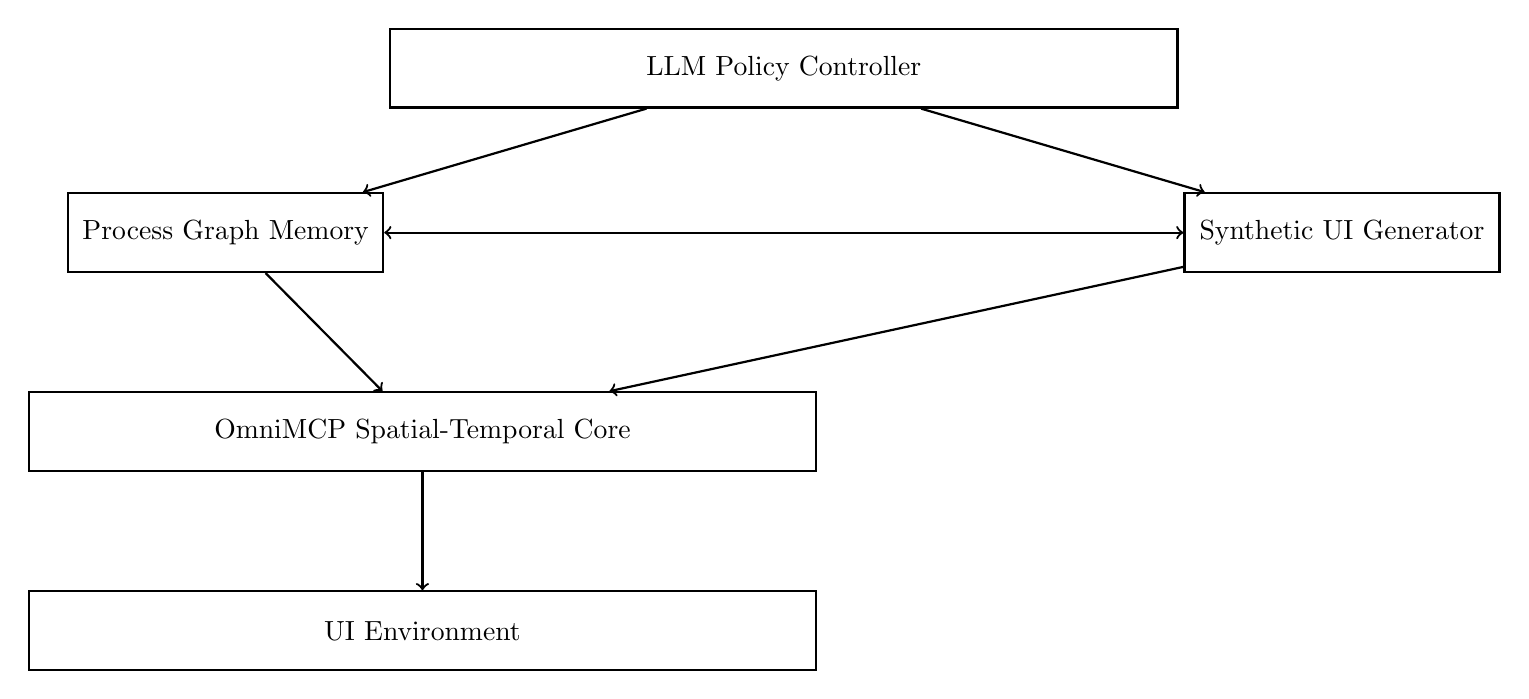
\begin{tikzpicture}[node distance=1.5cm, auto, thick]
    % Nodes
    \node[draw, rectangle, minimum width=10cm, minimum height=1cm] (llm) {LLM Policy Controller};
    \node[draw, rectangle, minimum width=4cm, minimum height=1cm, below left=of llm, xshift=1cm] (pg) {Process Graph Memory};
    \node[draw, rectangle, minimum width=4cm, minimum height=1cm, below right=of llm, xshift=-1cm] (sg) {Synthetic UI Generator};
    \node[draw, rectangle, minimum width=10cm, minimum height=1cm, below=of pg, xshift=2.5cm] (omni) {OmniMCP Spatial-Temporal Core};
    \node[draw, rectangle, minimum width=10cm, minimum height=1cm, below=of omni] (ui) {UI Environment};
    
    % Connections
    \draw[->] (llm) -- (pg);
    \draw[->] (llm) -- (sg);
    \draw[<->] (pg) -- (sg);
    \draw[->] (pg) -- (omni);
    \draw[->] (sg) -- (omni);
    \draw[->] (omni) -- (ui);
\end{tikzpicture}
\caption{Proposed RL-Enhanced OmniMCP Architecture}
\label{fig:rl-architecture}
\end{figure}

We envision formulating UI automation as a Markov Decision Process (MDP) where states are ScreenState objects, actions correspond to MCP tool operations, and rewards quantify interaction effectiveness. Rather than traditional RL algorithms, we propose Direct Preference Optimization (DPO) using LLMs to generate and evaluate interaction preferences.

Key components of this future enhancement would include:

\begin{enumerate}
    \item \textbf{Synthetic Data Generation}: Creating safe exploration spaces through LLM-generated UI variations, enabling the policy to learn from diverse scenarios without operational risks.
    
    \item \textbf{Process Graph-Augmented Memory}: Extending beyond the Markovian assumption to capture long-term patterns in successful UI interactions, storing embeddings of key states and retrieving similar interaction patterns when encountering familiar UI states.
    
    \item \textbf{LLM as Reward Function}: Employing the LLM itself as a contextualized reward function through structured evaluation prompts, considering progress toward goals, interaction efficiency, robustness, and safety.
    
    \item \textbf{Forecasting-Enhanced Exploration}: Introducing predictive modeling of future UI states resulting from potential action sequences, enabling mental simulation of multi-step interactions without execution.
\end{enumerate}

The training pipeline would consist of initialization from process graphs, refinement through synthetic UI interactions, and final tuning with limited real application interaction. This approach would enable OmniMCP to develop superhuman automation capabilities while maintaining interpretability and safety guarantees.

\begin{figure}[h]
\centering
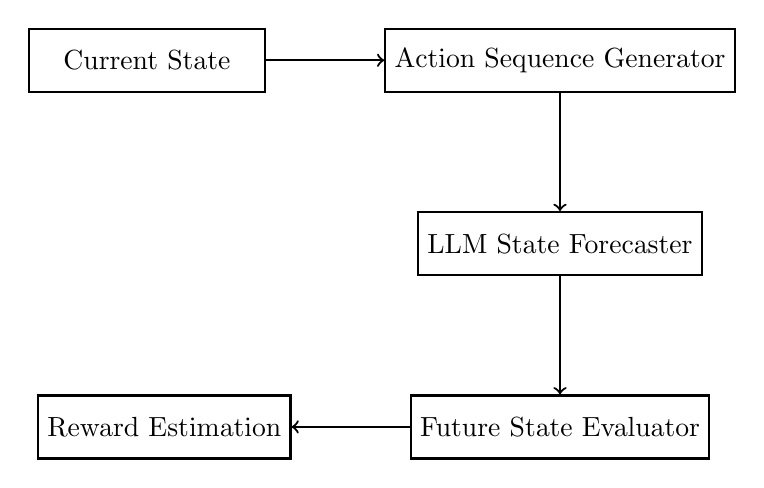
\begin{tikzpicture}[node distance=1.5cm, auto, thick]
    % Nodes
    \node[draw, rectangle, minimum width=3cm, minimum height=0.8cm] (current) {Current State};
    \node[draw, rectangle, minimum width=3cm, minimum height=0.8cm, right=of current] (gen) {Action Sequence Generator};
    \node[draw, rectangle, minimum width=3cm, minimum height=0.8cm, below=of gen] (forecast) {LLM State Forecaster};
    \node[draw, rectangle, minimum width=3cm, minimum height=0.8cm, below=of forecast] (eval) {Future State Evaluator};
    \node[draw, rectangle, minimum width=3cm, minimum height=0.8cm, left=of eval] (reward) {Reward Estimation};
    
    % Connections
    \draw[->] (current) -- (gen);
    \draw[->] (gen) -- (forecast);
    \draw[->] (forecast) -- (eval);
    \draw[->] (eval) -- (reward);
\end{tikzpicture}
\caption{Forecasting-Enhanced Exploration}
\label{fig:forecasting}
\end{figure}

\subsection{Additional Research Directions}

Beyond reinforcement learning integration, we plan to explore:
\begin{itemize}
    \item Development of comprehensive evaluation metrics
    \item Enhanced cross-platform generalization
    \item Integration with broader LLM architectures
    \item Collaborative multi-agent UI automation frameworks
\end{itemize}

\section{Conclusion}
We present OmniMCP as a significant advance in self-generating UI understanding. Through the synthesis of spatial and temporal features, coupled with robust prompt engineering and systematic validation capabilities, our framework demonstrates strong potential for generalizable UI automation. While further validation is needed, initial results suggest OmniMCP represents a meaningful step toward more robust and adaptable UI understanding systems.

\section{References}
[TODO]
\end{document}
